\documentclass[12pt,letterpaper]{article}

\usepackage{mathpazo}
\usepackage{fontspec}
\setmainfont{PatrickHand-Regular.ttf}[Path=./]
\usepackage[spanish,es-noshorthands]{babel}
\usepackage{amsmath,amssymb}
\usepackage{geometry}
\usepackage{graphicx}
\usepackage{float}
\usepackage{enumitem}
\usepackage{tikz}
\graphicspath{{figures/}}
\usepackage{xcolor}
\usepackage{eso-pic}

% Color de fondo estilo GoodNotes (blanco hueso muy suave)
\definecolor{gnbg}{HTML}{FDFDFD}
\pagecolor{gnbg}

% Color de "tinta" (un gris azulado oscuro para que parezca lápiz de tablet)
\definecolor{ink}{HTML}{2C3E50}
\color{ink}

% Dibujar cuadrícula estilo GoodNotes
\AddToShipoutPictureBG{%
  \begin{tikzpicture}[remember picture, overlay]
    \draw[step=6mm, color=gray!20, thin] (current page.south west) grid (current page.north east);
  \end{tikzpicture}
}

\geometry{margin=2.5cm}

\begin{document}

\begin{center}
  {\large \textbf{Solución de Ejercicios}}\\[0.3em]
  Probabilidad y Estadística
\end{center}

\bigskip

% ============================================================
\textbf{Ejercicio 1 — Cafetería de Facultad}
% ============================================================

\medskip
En una cafetería de facultad se atiende a 250 clientes. Se sabe que 30 consumen
té y leche, 40 consumen café y leche, 80 consumen leche, la unión té-leche es 130,
la unión café-leche es 150, y té con café no se intersectan. Determinar:
\begin{enumerate}[label=\alph*)]
  \item Probabilidad de que un cliente consuma solo té.
  \item Probabilidad de que un cliente consuma solo leche.
  \item Probabilidad de que consuma café dado que consume leche.
  \item Probabilidad de que no consuma ninguna de las tres bebidas.
\end{enumerate}

\medskip
\textit{Solución.}

Armamos el diagrama etiquetando cada zona. Como T y C no se intersectan,
los dos círculos laterales solo comparten área con L:

\begin{center}
\begin{tikzpicture}[scale=1]
  % --- circles: T(0,0) L(3,0) C(6,0) r=2 ---
  % T and C don't overlap (distance 6 > 4)
  \draw (0,0) circle (2);
  \draw (3,0) circle (2);
  \draw (6,0) circle (2);
  % Set labels — above each circle, clear of diagram
  \node[font=\small\bfseries] at ( 0, 2.35) {T};
  \node[font=\small\bfseries] at ( 3, 2.35) {L};
  \node[font=\small\bfseries] at ( 6, 2.35) {C};
  % Region letters — placed at geometric center of each zone
  % solo T: T spans [-2,2], L starts at 1 → solo T center ≈ (-0.5, 0)
  \node at (-0.7, 0) {$a$};
  % T∩L: overlap center at x=1.5 (midpoint of T-right=2 and L-left=1)
  \node at (1.5, 0)  {$b$};
  % solo L: between end of T-overlap(2) and start of C-overlap(4) → center 3
  \node at (3,   0)  {$c$};
  % L∩C: overlap center at x=4.5
  \node at (4.5, 0)  {$d$};
  % solo C: C spans [4,8], L ends at 5 → solo C center ≈ (6.5, 0)
  \node at (6.7, 0)  {$e$};
  % Bounding box
  \draw (-3,-2.6) rectangle (9,2.6);
  \node[font=\small] at (8.4, 2.2) {$f$};
\end{tikzpicture}
\end{center}

Asignamos: $a=$ solo T, $b=$ T$\cap$L, $c=$ solo L,
$d=$ C$\cap$L, $e=$ solo C, $f=$ ninguno.

De los datos leemos directamente: $b = 30$, $d = 40$.

Como $|L| = 80$:
\[
  b + c + d = 80 \;\Rightarrow\; c = 80 - 30 - 40 = 10
\]

Para $a$: como $|T \cup L| = 130$ y $|L| = 80$, $|T \cap L| = 30$:
\[
  |T| = 130 + 30 - 80 = 80 \;\Rightarrow\; a = 80 - 30 = 50
\]

Para $e$: de forma similar con $|C \cup L| = 150$:
\[
  |C| = 150 + 40 - 80 = 110 \;\Rightarrow\; e = 110 - 40 = 70
\]

Total dentro de algún conjunto: $50+30+10+40+70 = 200$, entonces $f = 250-200 = 50$.

\medskip
Con eso:
\begin{align*}
\text{a)}\quad P(\text{solo T}) &= \dfrac{50}{250} = 0.20 \\[6pt]
\text{b)}\quad P(\text{solo L}) &= \dfrac{10}{250} = 0.04 \\[6pt]
\text{c)}\quad P(C \mid L)      &= \dfrac{d}{b+c+d} = \dfrac{40}{80} = 0.50 \\[6pt]
\text{d)}\quad P(\text{ninguno})&= \dfrac{50}{250} = 0.20
\end{align*}

\bigskip

% ============================================================
\textbf{Ejercicio 2 — Partidos Políticos}
% ============================================================

\medskip
Dos partidos $A$ y $B$ compiten con $P(A)=0.53$ y $P(B)=0.47$.
Las probabilidades de implementar cada política según el ganador son:

\begin{center}
\begin{tabular}{lcc}
\hline
Política & $P(\cdot\mid A)$ & $P(\cdot\mid B)$ \\
\hline
Comercial (C)  & 0.47 & 0.12 \\
Defensa (D)    & 0.09 & 0.45 \\
Pensiones (P)  & 0.44 & 0.43 \\
\hline
\end{tabular}
\end{center}

\medskip
\textit{Solución.}

Usamos el árbol de probabilidad. Cada rama se multiplica a lo largo del recorrido
y luego se suman las ramas que llegan al mismo resultado:

\begin{figure}[H]
  \centering
  \begin{tikzpicture}[
    grow=right,
    level 1/.style={level distance=3.5cm, sibling distance=4cm},
    level 2/.style={level distance=5.5cm, sibling distance=1.5cm},
    hollow node/.style={circle,draw,inner sep=2pt,minimum size=6pt,fill=gnbg},
    rect node/.style={rectangle,draw,inner sep=4pt, fill=gnbg, text=ink, align=center},
    edge from parent/.style={draw, thin, -stealth},
    edge from parent path={(\tikzparentnode.east) -- (\tikzchildnode.west)}
  ]
  \node[hollow node] {}
    child { node[hollow node] {}
      child { node[rect node] {$P(P) = 0.43 \times 0.47 = 0.2021$} edge from parent node[pos=0.5, fill=gnbg, inner sep=1pt] {\footnotesize 0.43} }
      child { node[rect node] {$P(D) = 0.45 \times 0.47 = 0.2115$} edge from parent node[pos=0.5, fill=gnbg, inner sep=1pt] {\footnotesize 0.45} }
      child { node[rect node] {$P(C) = 0.12 \times 0.47 = 0.0564$} edge from parent node[pos=0.5, fill=gnbg, inner sep=1pt] {\footnotesize 0.12} }
      edge from parent node[pos=0.5, fill=gnbg, inner sep=1pt] {\footnotesize $P(B) = 0.47$}
    }
    child { node[hollow node] {}
      child { node[rect node] {$P(P) = 0.44 \times 0.53 = 0.2332$} edge from parent node[pos=0.5, fill=gnbg, inner sep=1pt] {\footnotesize 0.44} }
      child { node[rect node] {$P(D) = 0.09 \times 0.53 = 0.0477$} edge from parent node[pos=0.5, fill=gnbg, inner sep=1pt] {\footnotesize 0.09} }
      child { node[rect node] {$P(C) = 0.47 \times 0.53 = 0.2491$} edge from parent node[pos=0.5, fill=gnbg, inner sep=1pt] {\footnotesize 0.47} }
      edge from parent node[pos=0.5, fill=gnbg, inner sep=1pt] {\footnotesize $P(A) = 0.53$}
    };
  \end{tikzpicture}
\end{figure}

Sumando las ramas de cada política:
\begin{align*}
P(C) &= 0.2491 + 0.0564 = 0.3055 \\
P(D) &= 0.0477 + 0.2115 = 0.2592 \\
P(P) &= 0.2332 + 0.2021 = 0.4353
\end{align*}

\bigskip

% ============================================================
\textbf{Ejercicio 3 — Saturación de Carreras de Ingeniería}
% ============================================================

\medskip
Se encuestan $n=50$ egresados sobre saturación percibida del mercado laboral.
Construir tabla de frecuencias e histograma.

\medskip
\textit{Solución.}

\textbf{a) Tabla de frecuencias.}

\begin{center}
\begin{tabular}{lcccc}
\hline
Categoría    & $f_i$ & $f_{r}$ (\%) & $F_i$ & $F_{r}$ (\%) \\
\hline
Muy Baja     & 18 & 36 & 18 &  36 \\
Baja         &  9 & 18 & 27 &  54 \\
Media        & 10 & 20 & 37 &  74 \\
Saturada     & 11 & 22 & 48 &  96 \\
Muy Saturada &  2 &  4 & 50 & 100 \\
\hline
Total        & 50 & 100 & & \\
\hline
\end{tabular}
\end{center}

\medskip
\textbf{b) Histograma.}

\begin{center}
\begin{tikzpicture}[scale=0.9]
  \draw[->] (0,0) -- (0,4.2) node[above,font=\small] {$f_i$};
  \draw[->] (0,0) -- (11.5,0);
  % y ticks: scale 1 unit = 5
  \foreach \y/\val in {0.9/5, 1.8/10, 2.7/15, 3.6/20} {
    \draw (-0.1,\y) -- (0,\y);
    \node[left,font=\scriptsize] at (-0.1,\y) {\val};
  }
  % bars: heights = fi/5 * 0.9
  \foreach \x/\h/\fabs/\lbl in {
    0.4/3.24/18/Muy Baja,
    2.4/1.62/9/Baja,
    4.4/1.80/10/Media,
    6.4/1.98/11/Saturada,
    8.4/0.36/2/Muy Saturada} {
    \draw[fill=gray!25] (\x,0) rectangle (\x+1.8,\h);
    \node[above,font=\scriptsize] at (\x+0.9,\h) {\fabs};
    \node[below,rotate=35,anchor=north east,font=\scriptsize] at (\x+0.9,-0.1) {\lbl};
  }
\end{tikzpicture}
\end{center}

La categoría más frecuente es Muy Baja con 18 egresados (36\%).

\bigskip

% ============================================================
\textbf{Ejercicio 4 — Inmobiliaria BMU}
% ============================================================

\medskip
La inmobiliaria BMU registró superficies (mts$^2$) de $n=24$ departamentos.
Datos ordenados, rango $[59.1,\;121.8]$ mts$^2$.

\medskip
\textit{Solución.}

\textbf{a) Diagrama de caja y bigotes.}

Con $n=24$ datos, cada mitad tiene 12, entonces:
\begin{align*}
Q_1 &= \tfrac{1}{2}(x_{(6)}+x_{(7)}) = 65.1 \text{ mts}^2 \\
Q_2 &= \tfrac{1}{2}(x_{(12)}+x_{(13)}) = 69.8 \text{ mts}^2 \\
Q_3 &= \tfrac{1}{2}(x_{(18)}+x_{(19)}) = 83.6 \text{ mts}^2 \\
\text{RIC} &= 83.6 - 65.1 = 18.5 \text{ mts}^2
\end{align*}

Los límites del bigote son:
\begin{align*}
L_{\inf} &= 65.1 - 1.5(18.5) = 37.35 \text{ mts}^2 \\
L_{\sup} &= 83.6 + 1.5(18.5) = 111.35 \text{ mts}^2
\end{align*}

El bigote izquierdo llega a 59.1 y el derecho a 110.0.
Los valores 111.4 y 121.8 quedan fuera, son atípicos.

\begin{figure}[H]
  \centering
  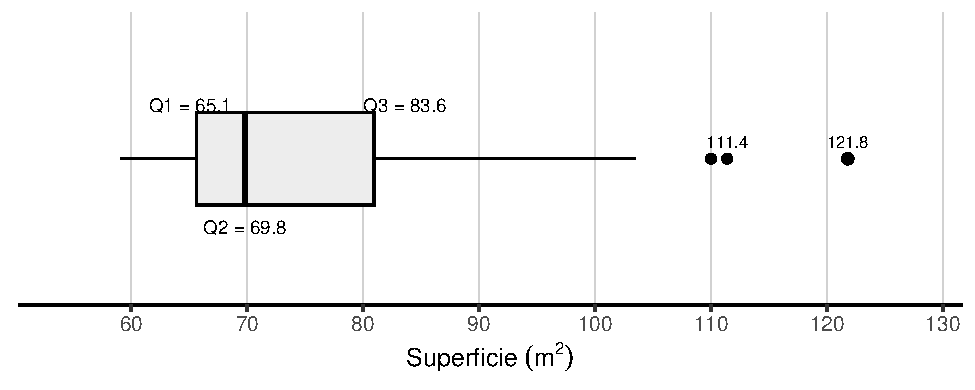
\includegraphics[width=0.88\textwidth]{boxplot_bmu.pdf}
\end{figure}

La distribución está sesgada a la derecha y tiene dos datos atípicos en el extremo superior.

\medskip
\textbf{b) Medidas de tendencia central.}

\[
  \bar{x} = 77.1\ \text{mts}^2, \qquad
  \tilde{x} = 69.8\ \text{mts}^2, \qquad
  \text{Moda: no existe}
\]

La mediana es la más representativa porque los outliers jalan la media hacia arriba.

\medskip
\textbf{c) Medidas de dispersión.}

\begin{align*}
R   &= 121.8 - 59.1 = 62.7\ \text{mts}^2 \\
S^2 &= 305.84\ \text{mts}^4 \\
S   &= \sqrt{305.84} \approx 17.49\ \text{mts}^2 \\
CV  &= \frac{17.49}{77.1}\times 100 \approx 22.7\%
\end{align*}

Un CV de 22.7\% indica dispersión moderada.

\medskip
\textbf{d) Transformación $Y = 1.04X + 3$.}

Con $Y = aX + b$, la media se transforma igual y la desviación solo escala con $a$:
\begin{align*}
\bar{y} &= 1.04(77.1) + 3 = 83.18\ \text{mts}^2 \\
S_Y     &= 1.04(17.49) = 18.19\ \text{mts}^2
\end{align*}

El $+3$ desplaza la distribución pero no afecta la dispersión.

\end{document}
